\begin{frame}{Methods for Electronic Dynamics}{By Propagation Algorithm}
    \textbf{Born-Oppenheimer Molecular Dynamics (BOMD)}
    \vspace{1em}
    
    \textbf{Car-Parrinello Molecular Dynamics (CPMD)}
    \vspace{1em}
    
    \textbf{Ehrenfest Molecular Dynamics(EMD)}
\end{frame}

\begin{frame}{Methods for Electronic Dynamics}{By Level of Electronic Theory}
    \begin{block}{Density Functional Theory (DFT-MD)}
    \end{block}
    
    \begin{block}{Wavefunction Theory (WFT-MD)}
        \textbf{Hartree-Fock (HF-MD)}
        \vspace{0.5em}
        
        \textbf{Post-Hartree-Fock (MP2-MD, CCSD-MD)}
    \end{block}
    
    \begin{block}{Semi-empirical Methods (SE-MD)}
    \end{block}
\end{frame}

%-----------------BOMD---------------------------- 

\begin{frame}{BOMD}
	\begin{block}{Paper Title}
  Born-Oppenheimer Molecular Dynamics	
	\end{block}
\end{frame}

\begin{frame}
    \frametitle{The Core Idea}
    \begin{columns}[T]
        \begin{column}{0.4\textwidth}
            \vspace{2cm}
            \begin{itemize}
                \item Nuclei are fixed. Electrons move.
                \item The huge mass difference is key.
            \end{itemize}
        \end{column}
        \begin{column}{0.5\textwidth}
            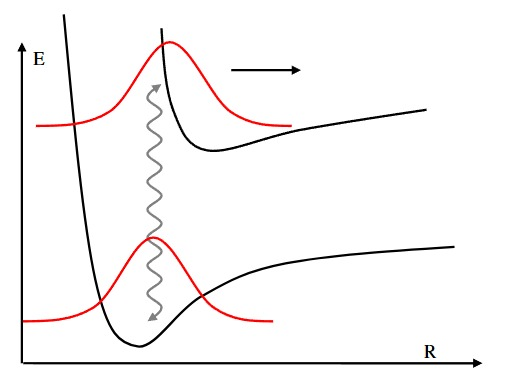
\includegraphics[width=\textwidth]{images/BO_app.png}
        \end{column}
    \end{columns}
\end{frame}

\begin{frame}
    \frametitle{The Result}
    \begin{columns}[T]
        \begin{column}{0.4\textwidth}
            \vspace{2cm}
            \begin{itemize}
                \item Defines the concept of molecular structure.
                \item It generates Potential Energy Surfaces (PES).
            \end{itemize}
        \end{column}
        \begin{column}{0.5\textwidth}
            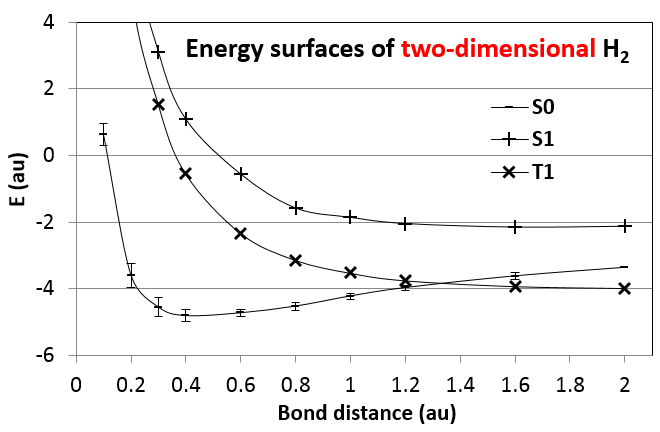
\includegraphics[width=\textwidth]{images/pot_ener_H2.png}
        \end{column}
    \end{columns}
\end{frame}

\begin{frame}
    \frametitle{The Limitation}
     \begin{columns}[T]
        \begin{column}{0.5\textwidth}
            \vspace{2cm}
            \begin{itemize}
                \item Fails when electronic states are coupled.
                \item Not suitable for most photochemical reactions.
            \end{itemize}
        \end{column}
        \begin{column}{0.45\textwidth}
            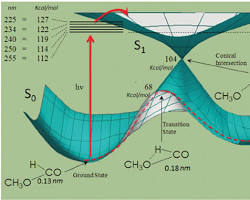
\includegraphics[width=\textwidth]{images/conic_intersect.png}
        \end{column}
    \end{columns}
\end{frame}

 %-----------------EMD---------------------------- 

\begin{frame}{EMD}
	\begin{block}{Paper Title}
	Ehrenfest Molecular Dynamics 
	\end{block}
\end{frame}

\begin{frame}
    \frametitle{The Core Idea}
     \begin{columns}[T]
        \begin{column}{0.5\textwidth}
            \vspace{2cm}
            \begin{itemize}
                \item Nuclei are treated as classical particles.
                \item Electrons are treated quantum mechanically.
            \end{itemize}
        \end{column}
        \begin{column}{0.5\textwidth}
            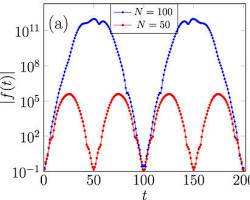
\includegraphics[width=\textwidth]{images/ehrenfest1.png}
        \end{column}
    \end{columns}
\end{frame}

\begin{frame}
    \frametitle{The Application}
    \begin{columns}[T]
        \begin{column}{0.5\textwidth}
            \vspace{2cm}
            \begin{itemize}
                \item Simulates non-adiabatic processes and transitions.
                \item Models molecular relaxation after photoexcitation.
            \end{itemize}
        \end{column}
        \begin{column}{0.5\textwidth}
            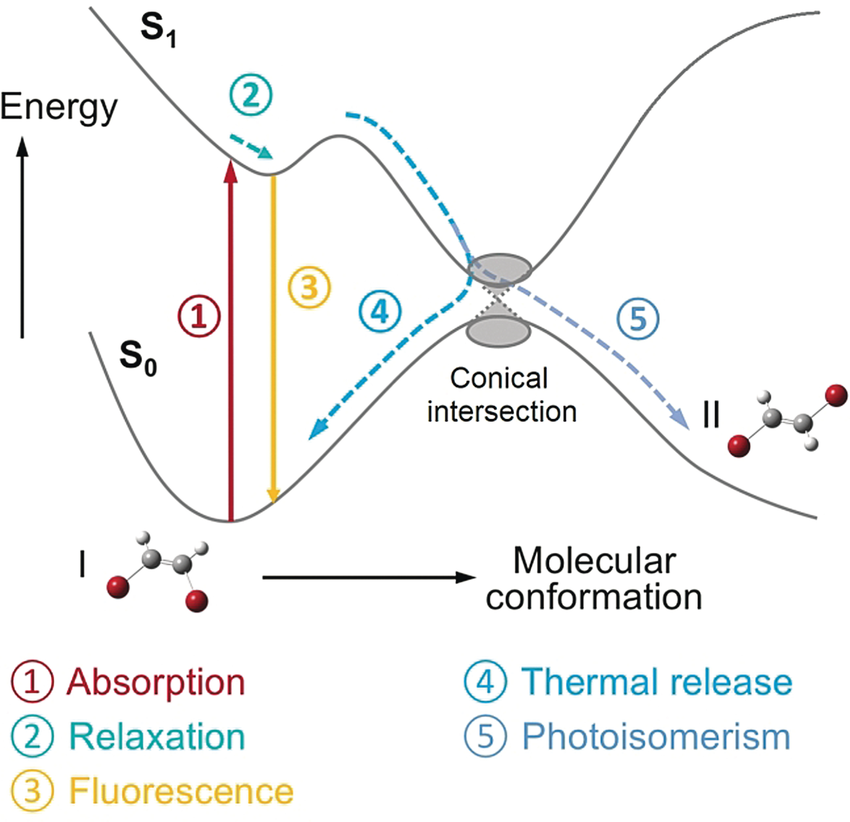
\includegraphics[width=\textwidth]{images/ehrenfest2.png}
        \end{column}
    \end{columns}
\end{frame}

\begin{frame}
    \frametitle{The Limitation}
    \begin{columns}[T]
        \begin{column}{0.5\textwidth}
            \vspace{2cm}
            \begin{itemize}
                \item It is a "mean-field" approximation.
                \item Fails to describe wavepacket branching.
            \end{itemize}
        \end{column}
        \begin{column}{0.5\textwidth}
            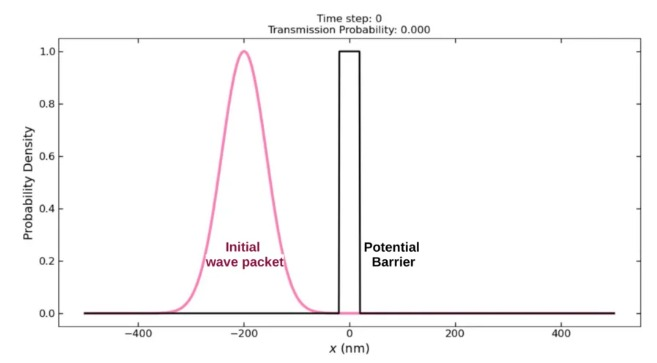
\includegraphics[width=\textwidth]{images/ehrenfest3.png}
        \end{column}
    \end{columns}
\end{frame}

%-----------------MP2---------------------------- 

\begin{frame}{MP2-MD}
	\begin{block}{Paper Title}
	Møller-Plesset Molecular Dynamics 
	\end{block}
\end{frame}

\begin{frame}
    \frametitle{The Core Idea}
    \begin{columns}[T]
        \begin{column}{0.5\textwidth}
            \vspace{2cm}
            \begin{itemize}
                \item Improves upon the Hartree-Fock method.
                \item Includes instantaneous electron correlation.
            \end{itemize}
        \end{column}
        \begin{column}{0.5\textwidth}
            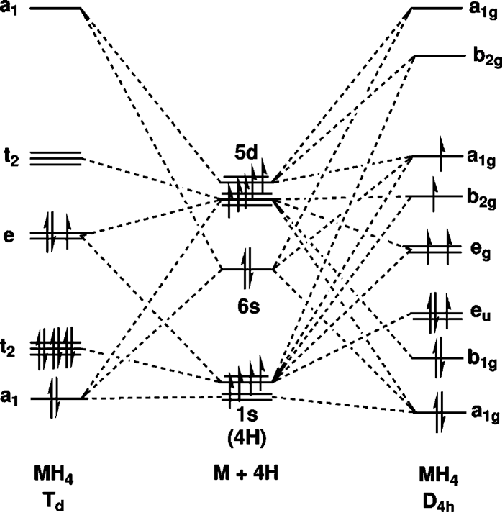
\includegraphics[width=\textwidth]{images/MP21.png}
        \end{column}
    \end{columns}
\end{frame}

\begin{frame}
    \frametitle{The Application}
     \begin{columns}[T]
        \begin{column}{0.4\textwidth}
            \vspace{2cm}
            \begin{itemize}
                \item Accurately describes van der Waals forces.
                \item Crucial for non-covalent interactions.
            \end{itemize}
        \end{column}
        \begin{column}{0.5\textwidth}
            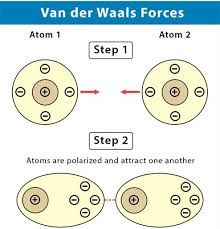
\includegraphics[width=\textwidth]{images/MP22.jpg}
        \end{column}
    \end{columns}
\end{frame}

\begin{frame}
    \frametitle{The Limitation}
    \begin{columns}[T]
        \begin{column}{0.45\textwidth}
            \vspace{2cm}
            \begin{itemize}
                \item Computationally expensive, scaling as N\textsuperscript{5}.
                \item Can fail for strongly correlated systems.
            \end{itemize}
        \end{column}
        \begin{column}{0.45\textwidth}
            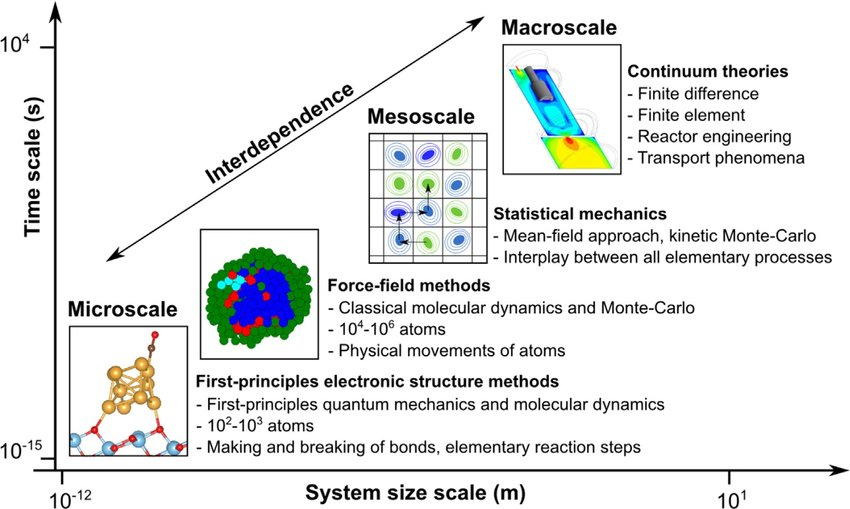
\includegraphics[width=\textwidth]{images/MP23.png}
        \end{column}
    \end{columns}
\end{frame}

\begin{frame}
    \frametitle{Water simulation with MP2}
     \begin{columns}[T]
        \begin{column}{0.5\textwidth}
            \vspace{2cm}
            \begin{itemize}
                \item First ab initio MD of water with MP2.
                \item Overcame immense computational cost.
            \end{itemize}
        \end{column}
        \begin{column}{0.5\textwidth}
            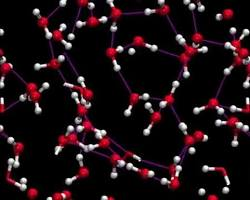
\includegraphics[width=\textwidth]{images/waterMP21.jpg}
            \tiny{\url{https://youtu.be/Zl74NCVbA5A?si=_vw8W1vdoYTN6lkV}}
        \end{column}
    \end{columns}
\end{frame}

\begin{frame}
    \frametitle{The Result}
    \begin{columns}[T]
        \begin{column}{0.5\textwidth}
            \vspace{2cm}
            \begin{itemize}
                \item Produced a more realistic water structure.
                \item Matched experimental RDF data better.
            \end{itemize}
        \end{column}
        \begin{column}{0.5\textwidth}
            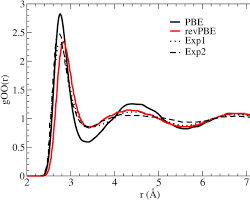
\includegraphics[width=\textwidth]{images/waterMP22.png}
        \end{column}
    \end{columns}
\end{frame}

\begin{frame}
    \frametitle{The Impact}
    \begin{columns}[T]
        \begin{column}{0.5\textwidth}
            \vspace{2cm}
            \begin{itemize}
                \item Set a new benchmark for DFT methods.
                \item Proved correlation is essential for water.
            \end{itemize}
        \end{column}
        \begin{column}{0.5\textwidth}
            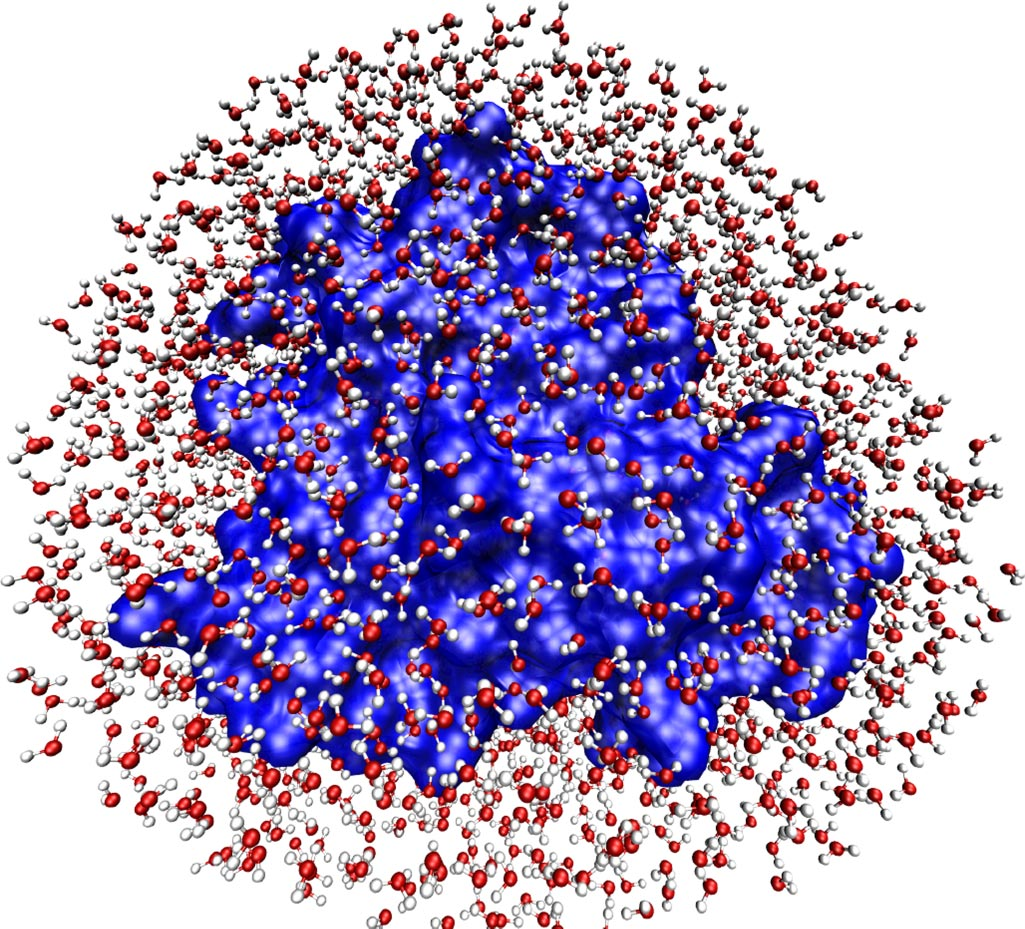
\includegraphics[width=\textwidth]{images/waterMP23.png}
        \end{column}
    \end{columns}
\end{frame}

%-----------------CCSD---------------------------- 

\begin{frame}{CCSD-MD}
	\begin{block}{Paper Title}
	Coupled Cluster Singles and Doubles Molecular Dynamics
	\end{block}
\end{frame}

\begin{frame}
    \frametitle{The Method}
    \begin{columns}[T]
        \begin{column}{0.5\textwidth}
            \vspace{2cm}
            \begin{itemize}
                \item Uses Machine Learning for MD simulations.
                \item Achieves "gold standard" CCSD(T) accuracy.
            \end{itemize}
        \end{column}
        \begin{column}{0.45\textwidth}
            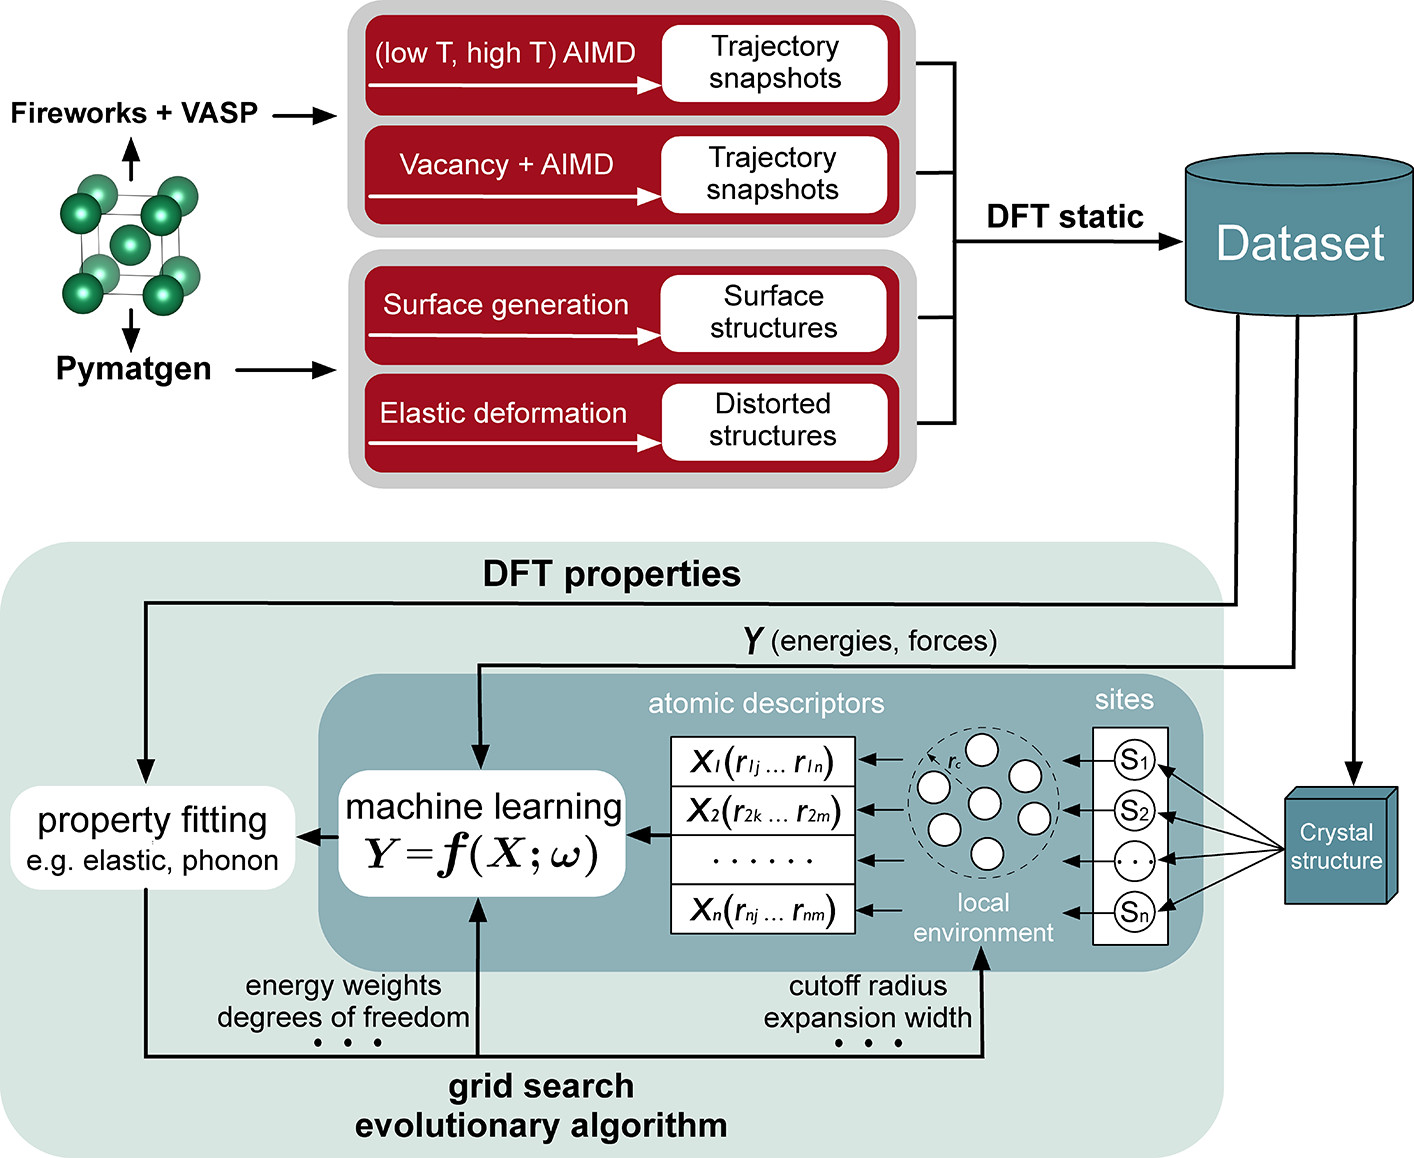
\includegraphics[width=\textwidth]{images/CCSD(T)1.jpeg}
        \end{column}
    \end{columns}
\end{frame}

\begin{frame}
    \frametitle{The Result}
    \begin{columns}[T]
        \begin{column}{0.5\textwidth}
            \vspace{2cm}
            \begin{itemize}
                \item Accurately reproduced water's phase diagram.
                \item Captured water's famous density anomaly.
            \end{itemize}
        \end{column}
        \begin{column}{0.5\textwidth}
            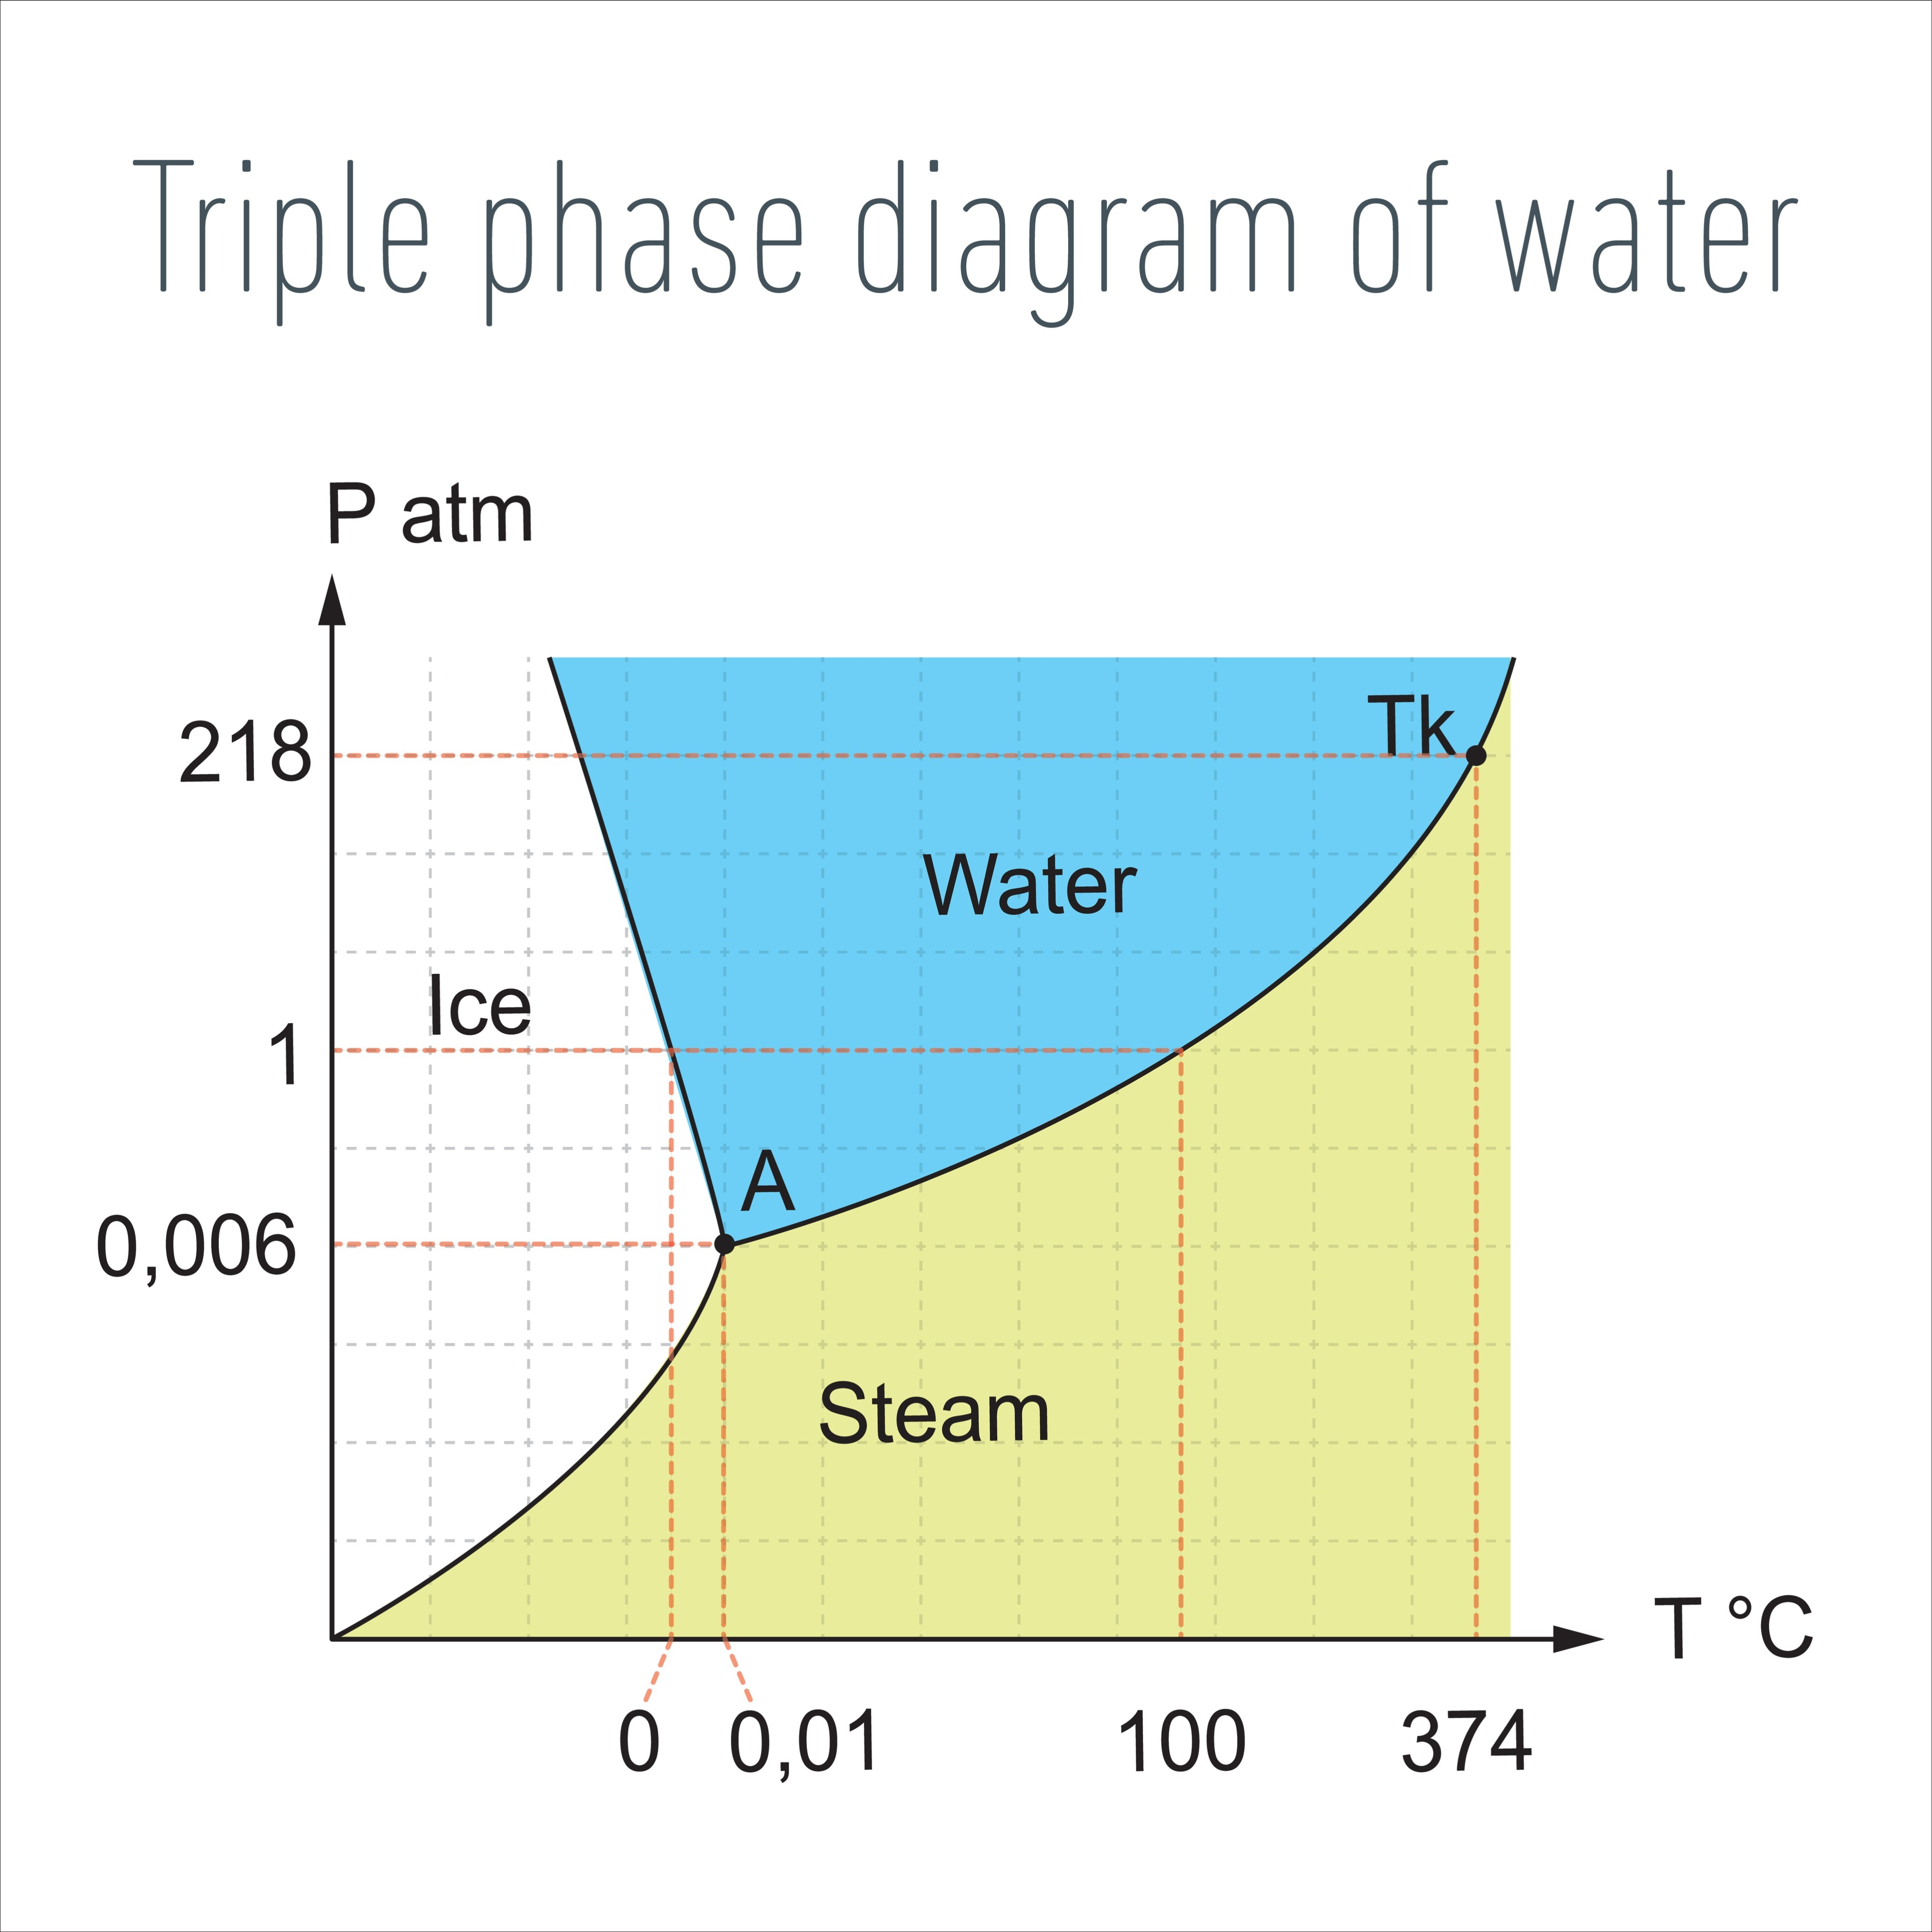
\includegraphics[width=\textwidth]{images/CCSD(T)2.jpg}
        \end{column}
    \end{columns}
\end{frame}

\begin{frame}
    \frametitle{The Future}
    \begin{columns}[T]
        \begin{column}{0.5\textwidth}
            \vspace{2cm}
            \begin{itemize}
                \item Revolutionizing simulations in materials science.
                \item Enables gold-standard accuracy for large systems.
            \end{itemize}
        \end{column}
        \begin{column}{0.5\textwidth}
            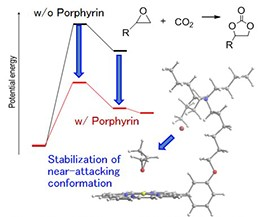
\includegraphics[width=\textwidth]{images/CCSD(T)3.jpg}
        \end{column}
    \end{columns}
\end{frame}


\subsection{Semi-Epirical (MNDO, AM1, Tight-Bending)}

%-----------------MNDO----------------------------

\begin{frame}{MNDO}
	\begin{block}{Paper Title}
	Ground State of Molecules The MNDO Method Approximation and Parameters
	\end{block}
\end{frame}

\begin{frame}{The MNDO method}
    \begin{block}{Objective}
        To develop a fast and reliable quantum method for predicting molecular properties.
    \end{block}
    \pause
    
    \begin{itemize}
        \item It is a \textbf{semiempirical} method, meaning it combines theory with experimental parameters.
        \pause
        \bigskip
        \item Its theoretical basis is the \textbf{NDDO} (Neglect of Diatomic Differential Overlap) approximation, which is more rigorous than previous methods like INDO or CNDO.
    \end{itemize}
\end{frame}



\begin{frame}{Approximation I: One-Center Terms}
    \begin{block}{Energies and Repulsions on a Single Atom}
        \begin{itemize}
            \item The terms that describe the energy of an electron in an atom ($U_{\mu\mu}$) and the repulsion between electrons on the same atom ($g_{\mu\nu}$, $h_{\mu\nu}$) are not calculated theoretically.
            \pause
            \bigskip
            \item Instead, they are derived by fitting the calculations to \textbf{experimental spectroscopic data} for the atom and its ions.
            \pause
            \bigskip
            \item This implicitly introduces an \textbf{electron correlation} effect, as the fitted values are smaller than the theoretical ones.
        \end{itemize}
    \end{block}
\end{frame}



\begin{frame}{Approximation II: Two-Center Repulsion}
    \begin{alertblock}{The Key Innovation of MNDO}
        The repulsion between the charge distribution of an atom A and another atom B is modeled classically.
    \end{alertblock}
    \pause
    
    \begin{itemize}
        \item The interaction is decomposed into a sum of interactions between \textbf{multipoles} (monopole, dipole, quadrupole).
        \pause
        \bigskip
        \item Each multipole is in turn represented as a simple configuration of \textbf{point charges}.
        \pause
        \bigskip
        \item The final repulsion energy is calculated by summing the interactions between these point charges using a semiempirical formula.
    \end{itemize}
\end{frame}



\begin{frame}{Approximation III: Chemical Bonding}
    \begin{block}{Core-Core and Resonance Interactions}
        \begin{itemize}
            \item \textbf{Core-Core Repulsion:} The repulsion between the nuclei and inner-shell electrons ("cores") is modeled with a function that blends charge repulsion with an adjustable exponential term.
            \pause
            \bigskip
            \item \textbf{Resonance Integrals ($\beta_{\mu\lambda}$):} These are responsible for most of the bonding energy. They are assumed to be proportional to the overlap of the atomic orbitals, with a constant that depends on atomic parameters.
        \end{itemize}
    \end{block}
\end{frame}



\begin{frame}{The Parametrization Process}
    \begin{block}{Fitting to Experimental Reality}
        \begin{itemize}
            \item The mathematical expressions in the method contain a series of \textbf{atomic parameters} ($\zeta, U_{ss}, \beta_p$, etc.).
            \pause
            \bigskip
            \item The values of these parameters are not derived from theory. They are obtained through a \textbf{nonlinear least-squares optimization process}.
            \pause
            \bigskip
            \item The parameters are adjusted until the calculated properties (heats of formation, geometries, etc.) for a set of standard molecules match their \textbf{experimental values} as closely as possible.
        \end{itemize}
    \end{block}
\end{frame}

%-------------AM1------------------------------------------

\begin{frame}{AM1}
	\begin{block}{Paper Title}
	AM1: A New Method General Purpose Quantum Mechanical Molecular Model
	\end{block}
\end{frame}

\begin{frame}
  \frametitle{AM1 - Austin Model 1}
  
  \begin{itemize}
    \item \textbf{Austin Model 1 (AM1)} is a semiempirical quantum mechanical molecular model developed in the mid-80s by Michael J. S. Dewar's group. \pause
    \item \textbf{Objective:} To be a general-purpose computational tool for studying: \pause
    \begin{itemize}
        \item Large molecular systems. \pause
        \item Chemical reactions and their mechanisms. \pause
    \end{itemize}
    \item It was created as an alternative to \textit{ab initio} methods, which were prohibitively expensive in terms of computation time for molecules of real chemical interest.
  \end{itemize}
\end{frame}

\begin{frame}
  \frametitle{The Predecessor: Weaknesses of MNDO}
  
  AM1 is a direct evolution of the MNDO (\textit{Modified Neglect of Diatomic Overlap}) method and was designed to correct its most significant flaws: \pause
  
  \begin{block}{Main Flaws of MNDO}
    \begin{itemize}
      \item Inability to correctly reproduce \textbf{hydrogen bonds}. \pause
      \item Overestimation of interatomic repulsions, leading to errors in: \pause
      \begin{itemize}
          \item Sterically hindered molecules (e.g., neopentane). \pause
          \item Molecules with four-membered rings. \pause
      \end{itemize}
      \item A tendency to calculate activation energies that were too high.
    \end{itemize}
  \end{block}
\end{frame}


\begin{frame}
  \frametitle{Methodology and Key Improvements}
  
  \begin{itemize}
    \item AM1 is based on the same approximation as MNDO: \textbf{Neglect of Diatomic Differential Overlap (NDDO)}. \pause
    \item \textbf{Key Modification:} The \textbf{Core Repulsion Function (CRF)} was optimized. \pause
    \begin{itemize}
        \item \textbf{Gaussian terms} were added to the MNDO function. \pause
        \item This allows for the adjustment of interatomic repulsions to improve the description of medium and long-range interactions. \pause
    \end{itemize}
    \item The parameters for the elements C, H, O, and N were optimized simultaneously, using a larger dataset and an improved optimization procedure.
  \end{itemize}
\end{frame}

% --- Slide on Results and Advantages ---
\begin{frame}
  \frametitle{Results and Advantages of AM1}
  
  AM1 proved to be a substantial improvement over MNDO without increasing computation time. \pause
  
  \begin{alertblock}{Main Advantages}
    \begin{itemize}
      \item<2-> Capable of genuinely modeling \textbf{hydrogen bonds}. \pause
      \item<3-> More accurate estimates of \textbf{activation energies}. \pause
      \item<4-> Better treatment of \textbf{hindered molecules} (e.g., neopentane) and those with ring strain (e.g., cubane).
    \end{itemize}
  \end{alertblock}
  
\end{frame}

%------------------------Tight-Bending---------------------

\begin{frame}{Tight-Bending}
	\begin{block}{Paper Title}
	Self-consistent-charge density-functional tight-binding method for simulations of complex
materials properties
	\end{block}
\end{frame}

\begin{frame}
  \frametitle{The Limits of Standard Tight-Binding}
  
  Standard Tight-Binding (TB) is a computationally fast method derived from Density-Functional Theory (DFT). \pause
  
  \begin{itemize}
    \item It works well when the charge density of a system can be approximated as a simple superposition of neutral atom densities. \pause
    
    \item However, it has a significant limitation: it is a \textbf{non-self-consistent} method. \pause
    
    \item This means it cannot account for the transfer of charge between different types of atoms. This leads to failures in polar or heteronuclear systems and limits the method's overall transferability.
  \end{itemize}
\end{frame}

\begin{frame}
  \frametitle{The SCC-DFTB Solution: Self-Consistent Charges}
  
  The Self-Consistent-Charge (SCC) method extends the standard approach by allowing the system's charges to re-distribute. \pause
  
  \begin{block}{The Core Principle}
    It is based on a second-order expansion of the DFT total energy with respect to fluctuations in the charge density ($\delta n$).
  \end{block} \pause
  
  \begin{itemize}
    \item A new energy term is added that depends on the Mulliken charge fluctuations ($\Delta q$) on each atom. \pause
    
    \item This term correctly describes long-range Coulomb interactions between charges and includes on-site self-interaction effects related to an atom's chemical hardness (the Hubbard parameter U). \pause
    
    \item The method then iterates, adjusting the charges and recalculating the energy until a self-consistent, minimum-energy solution is found.
  \end{itemize}
\end{frame}

\begin{frame}
  \frametitle{Why It Matters: The Payoff of SCC-DFTB}
  
  This self-consistent charge correction makes the method significantly more accurate and robust. \pause
  
  \begin{alertblock}{Key Advantages}
    \begin{itemize}
      \item \textbf{Enhanced Transferability:} By properly treating charge transfer, the method is successfully applied to a much broader range of systems, including polar molecules, semiconductors, and large biomolecules. \pause
      
      \item \textbf{Improved Accuracy:} It leads to a considerable improvement in total energies, forces, vibrational frequencies, and molecular geometries compared to the non-SCC approach. \pause
      
      \item \textbf{Efficiency is Maintained:} The self-consistent cycle is very fast, typically converging in just 3-5 iterations. The method remains orders of magnitude faster than ab initio calculations.
    \end{itemize}
  \end{alertblock}
  
\end{frame}

\subsection{Post-Hartree-Fock (MP2-MD, CCSD-MD)}

%--------------------------CCSD------------------

\begin{frame}{CCSD-MD}
	\begin{block}{Paper Title}
	On the Correlation Problem in Atomic and Molecular Systems. Calculation of Wavefunction Components in Ursell-Type Expansion Using Quantum Field Theoretical Methods 
	\end{block}
\end{frame}


\begin{frame}{Coupled Cluster (CC) Method}
    \begin{block}{The Problem: Electron Correlation}
        Standard methods like Hartree-Fock ignore that electron movements are correlated. The CC method aims to calculate this \textbf{correlation energy}.
    \end{block}
    \pause

    \begin{alertblock}{The Central Idea: The Exponential Ansatz}
        It expresses the exact wavefunction $|\Psi\rangle$ by applying an exponential "cluster operator" $e^{\hat{T}}$ to the Hartree-Fock wavefunction $|\Phi\rangle$:
        \[
        |\Psi\rangle = e^{\hat{T}} |\Phi\rangle
        \]
    \end{alertblock}
\end{frame}

%------------------------------------------------

\begin{frame}{How Coupled Cluster Works}
    \begin{itemize}
        \item The \textbf{cluster operator} $\hat{T}$ is a sum of excitation operators ($\hat{T} = \hat{T}_1 + \hat{T}_2 + \dots$), where $\hat{T}_1$ creates single excitations, $\hat{T}_2$ creates double excitations, and so on.
        \pause
        \bigskip
        \item The method uses tools from \textbf{quantum field theory} (hole-particle formalism, Wick's theorem) to solve for the amplitudes of these excitations.
        \pause
        \bigskip
        \item Its key advantage over Configuration Interaction (CI) is that truncating at $\hat{T}_2$ (CCSD) still includes the most important effects of quadruple excitations, making the method very efficient and \textbf{size-extensive}.
    \end{itemize}
\end{frame}

\begin{frame}{CCSD vs GCCSD}
    \begin{figure}
        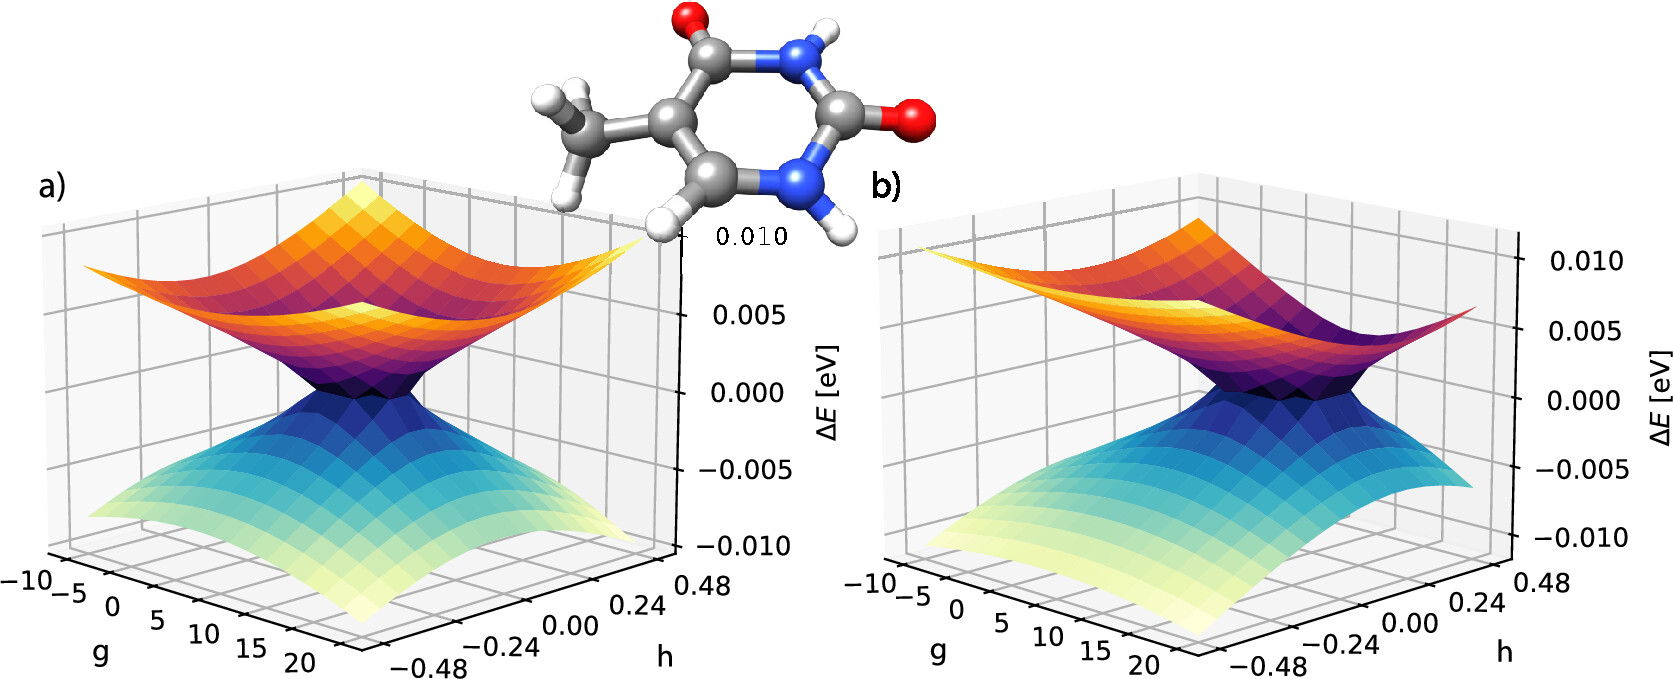
\includegraphics[width=0.8\textwidth]{images/CCSD.jpeg}
        \caption{Superficies de energía potencial S1 y S2 en timina calculadas con CCSD (a) y GCCSD (b).}
    \end{figure}
\end{frame}
